% --- UNIVERSAL PREAMBLE BLOCK ---
\documentclass[11pt, a4paper]{article}

\usepackage[utf8]{inputenc}
\usepackage[T1]{fontenc}
\usepackage[spanish, es-tabla, es-nodecimaldot]{babel}
\usepackage[a4paper, top=2.5cm, bottom=2.5cm, left=2.5cm, right=2.5cm]{geometry}

\usepackage{graphicx}
\usepackage{float}
\usepackage{hyperref}
\usepackage{enumitem}
\usepackage{xcolor}
\usepackage{listings}
\usepackage{fancyhdr}
\usepackage{tabularx}
\usepackage{longtable}
\usepackage{xltabular}
\usepackage{booktabs}
\usepackage{colortbl}
\usepackage{caption}
\usepackage{amssymb}

\setlist[itemize]{label=-}
\setcounter{secnumdepth}{0}

\definecolor{codegreen}{rgb}{0,0.6,0}
\definecolor{codegray}{rgb}{0.5,0.5,0.5}
\definecolor{codepurple}{rgb}{0.58,0,0.82}
\definecolor{backcolour}{rgb}{0.96,0.96,0.96}

\lstdefinestyle{pythonstyle}{
    backgroundcolor=\color{backcolour},
    commentstyle=\color{codegreen},
    keywordstyle=\color{magenta},
    numberstyle=\tiny\color{codegray},
    stringstyle=\color{codepurple},
    basicstyle=\ttfamily\small,
    breakatwhitespace=false,
    breaklines=true,
    captionpos=b,
    keepspaces=true,
    numbers=left,
    numbersep=5pt,
    showspaces=false,
    showstringspaces=false,
    showtabs=false,
    tabsize=4,
    language=Python,
    extendedchars=true,
    literate={á}{{\'a}}1 {é}{{\'e}}1 {í}{{\'i}}1 {ó}{{\'o}}1 {ú}{{\'u}}1 {ñ}{{\~n}}1 {Á}{{\'A}}1 {É}{{\'E}}1 {Í}{{\'I}}1 {Ó}{{\'O}}1 {Ú}{{\'U}}1 {Ñ}{{\~N}}1 {π}{{$\pi$}}1 {²}{{$^2$}}1 {³}{{$^3$}}1 {¿}{{?`}}1
}
\lstset{style=pythonstyle}

\hypersetup{
    colorlinks=true,
    linkcolor=black,
    filecolor=magenta,
    urlcolor=blue,
    pdftitle={Actividad 3 - POO},
}

% Comando auxiliar para dibujar un cuadro de clase estilo UML
\newcommand{\clasebox}[3]{%
\begin{center}
\begin{tabular}{|l|}
\hline
\textbf{#1} \\
\hline
#2
\hline
#3
\hline
\end{tabular}
\end{center}
}

% Comando auxiliar para dibujar un objeto estilo UML (nombre subrayado)
\newcommand{\objetobox}[2]{%
\begin{center}
\begin{tabular}{|l|}
\hline
\underline{\textbf{#1}} \\
\hline
#2
\hline
\end{tabular}
\end{center}
}

\begin{document}

% ---------------------------------------------------------
% PORTADA
% ---------------------------------------------------------
\begin{titlepage}
    \centering
    \vspace*{1cm}

    {\huge \textbf{Universidad Nacional de Colombia}\par}
    \vspace{0.5cm}
    {\Large Facultad de Minas\par}
    \vspace{1.5cm}

    {\Large \textbf{Programación Orientada a Objetos 2026-2}\par}
    \vspace{2cm}

    {\huge \textbf{Actividad 3}\par}
    \vspace{0.5cm}
    {\large Interfaces gráficas de usuario y herencia: solución de los ejercicios 8.2 y 8.3\par}

    \vspace{3cm}

    \textbf{Presentado por:}\par
    \vspace{0.5cm}
    {\Large \textbf{Natalia Patricia Remolina Rodríguez}\par}

    \vspace{2cm}

    \textbf{Docente:}\par
    Walter Hugo Arboleda Mazo\par

    \vspace{2cm}

    Medellín, Colombia\par
    22 de octubre de 2026
\end{titlepage}

% ---------------------------------------------------------
% EJERCICIO 3.1
% ---------------------------------------------------------
\section{Ejercicio 8.2. Componentes swing: Notas}

\subsection{Enunciado}
Se requiere desarrollar un programa con interfaz gráfica de usuario que genere una ventana
donde se solicite el ingreso de cinco notas obtenidas por un estudiante. El programa debe
calcular y mostrar en la parte inferior de la ventana los siguientes datos:

\begin{itemize}
    \item El promedio de las notas ingresadas.
    \item La desviación estándar de las notas ingresadas.
    \item La mayor nota obtenida.
    \item La menor nota obtenida.
\end{itemize}

\noindent \textbf{Ejercicios propuestos incluidos en la solución:}
\begin{itemize}
    \item Generar mensajes de alerta cuando se ingresen datos que no sean numéricos.
    \item Es obligatorio ingresar las cinco notas: se genera un mensaje de alerta cuando
          alguna nota no ha sido ingresada.
\end{itemize}

\noindent \textbf{Enlace al repositorio en GitHub:} \\
\url{https://github.com/NatoRemolina/UNAL-Programacion-Orientada-a-Objetos/blob/main/actividad-03/ejercicio1.py}

\subsection{Diagrama de clases}
\clasebox{Notas}
{%
- notas \\
}
{%
+ calcular\_promedio() \\
+ calcular\_desviacion\_estandar() \\
+ calcular\_mayor() \\
+ calcular\_menor() \\
}

\clasebox{VentanaNotas}
{%
- color\_fondo \\
- color\_texto \\
- entradas\_notas \\
- lbl\_promedio \\
- lbl\_desviacion \\
- lbl\_mayor \\
- lbl\_menor \\
}
{%
+ \_crear\_componentes() \\
+ action\_calcular() \\
+ action\_limpiar() \\
}

\noindent \textbf{Relaciones:}
\begin{itemize}
    \item \texttt{VentanaNotas} hereda de \texttt{tk.Tk}: es la ventana principal de la aplicación.
    \item \texttt{VentanaNotas} usa a \texttt{Notas} (dependencia): crea un objeto de esa clase cada
          vez que se presiona el botón \textit{Calcular} y le delega los cálculos. De esta forma la
          lógica del negocio queda separada de la presentación.
\end{itemize}

\newpage
\subsection{Diagrama de objetos}
El siguiente diagrama corresponde al estado de la aplicación en el momento en que se ingresan
las notas 5.0, 3.5, 2.5, 4.5 y 3.6 y se presiona el botón \textit{Calcular}.

\objetobox{ventana : VentanaNotas}
{%
color\_fondo = "\#e3f2fd" \\
color\_texto = "\#0d47a1" \\
entradas\_notas = [5.0, 3.5, 2.5, 4.5, 3.6] \\
}

\objetobox{calculadora : Notas}
{%
notas = [5.0, 3.5, 2.5, 4.5, 3.6] \\
}

\noindent El objeto \texttt{ventana} mantiene una referencia temporal a \texttt{calculadora}
mientras dura el cálculo, y con los valores que este retorna actualiza sus etiquetas:
promedio = 3.82, desviación estándar = 0.87, mayor nota = 5.00 y menor nota = 2.50.

\subsection{Casos de uso}
\begin{table}[H]
\centering
\begin{tabularx}{\textwidth}{@{}l X@{}}
\toprule
\textbf{Caso de uso} & CU-01: Calcular los indicadores estadísticos \\
\midrule
\textbf{Actor} & Usuario (docente o estudiante) \\
\textbf{Precondición} & La ventana de la calculadora está abierta. \\
\textbf{Flujo principal} & 1. El usuario ingresa las cinco notas. \newline
                           2. El usuario presiona el botón \textit{Calcular}. \newline
                           3. El sistema valida que las cinco casillas estén diligenciadas. \newline
                           4. El sistema valida que todos los valores sean numéricos. \newline
                           5. El sistema calcula promedio, desviación estándar, mayor y menor. \newline
                           6. El sistema muestra los cuatro resultados en la parte inferior. \\
\textbf{Flujo alterno A} & En el paso 3, si alguna casilla está vacía, el sistema muestra la
                           alerta \textit{"Es obligatorio ingresar las cinco notas"} e indica
                           cuáles faltan. El caso de uso termina. \\
\textbf{Flujo alterno B} & En el paso 4, si algún valor no es numérico, el sistema muestra la
                           alerta \textit{"Por favor, ingrese números válidos"}. El caso de uso termina. \\
\textbf{Postcondición} & Los cuatro indicadores quedan visibles en la ventana. \\
\bottomrule
\end{tabularx}
\end{table}

\begin{table}[H]
\centering
\begin{tabularx}{\textwidth}{@{}l X@{}}
\toprule
\textbf{Caso de uso} & CU-02: Limpiar el formulario \\
\midrule
\textbf{Actor} & Usuario \\
\textbf{Precondición} & La ventana de la calculadora está abierta. \\
\textbf{Flujo principal} & 1. El usuario presiona el botón \textit{Limpiar}. \newline
                           2. El sistema borra el contenido de las cinco casillas. \newline
                           3. El sistema restablece las cuatro etiquetas de resultados. \\
\textbf{Postcondición} & La ventana queda en su estado inicial, lista para un nuevo cálculo. \\
\bottomrule
\end{tabularx}
\end{table}

\newpage
\subsection{Interfaz de usuario}

\begin{figure}[H]
    \centering
    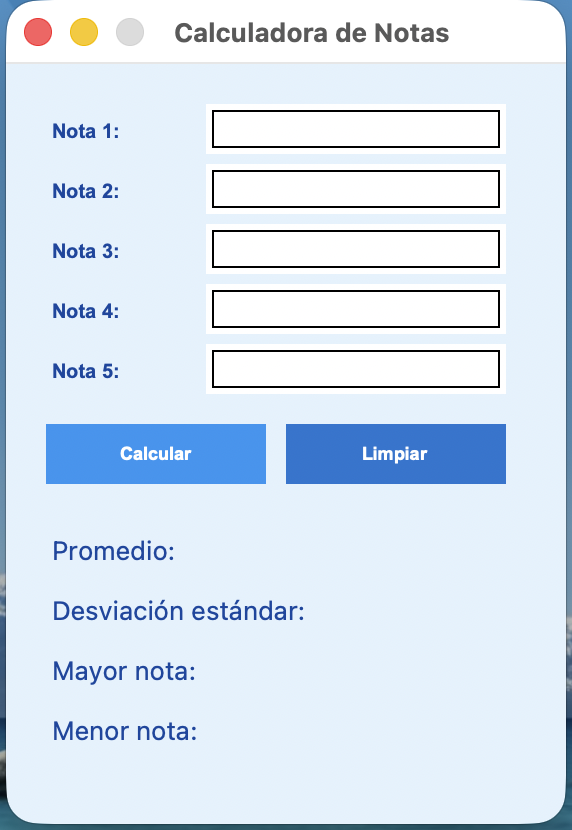
\includegraphics[width=0.42\textwidth]{img/notas_inicial.png}
    \hspace{0.04\textwidth}
    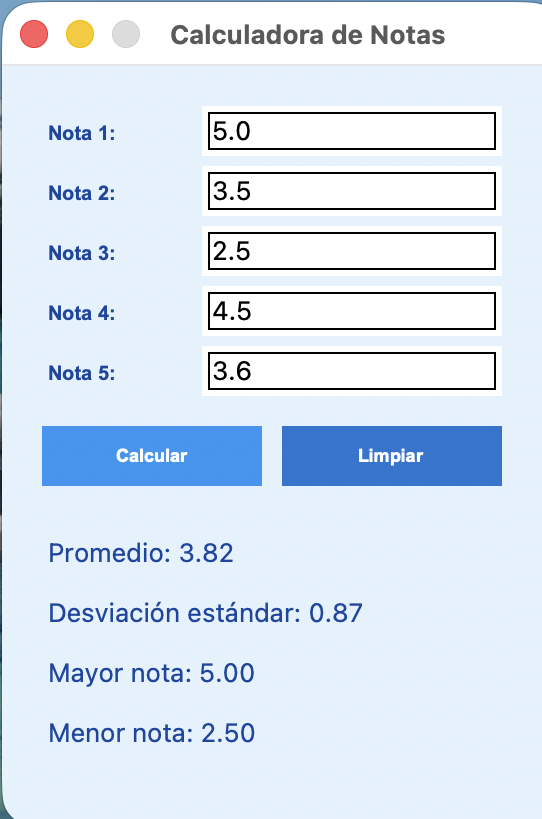
\includegraphics[width=0.42\textwidth]{img/notas_resultado.png}
    \caption{Ventana principal al iniciar la aplicación (izquierda) y resultado del
             procesamiento de las cinco notas (derecha).}
\end{figure}

% ---------------------------------------------------------
% NOTA: aquí van las dos capturas de las ventanas de alerta.
% Guarde sus imágenes en la carpeta img/ con estos nombres y
% elimine el signo % de las cuatro líneas siguientes.
% ---------------------------------------------------------
% \begin{figure}[H]
%     \centering
%     \includegraphics[width=0.45\textwidth]{img/notas_alerta_incompletos.png}
%     \hspace{0.04\textwidth}
%     \includegraphics[width=0.45\textwidth]{img/notas_alerta_texto.png}
%     \caption{Alertas de los ejercicios propuestos: notas faltantes y datos no numéricos.}
% \end{figure}

\subsection{Código fuente}
\begin{lstlisting}
import tkinter as tk
from tkinter import messagebox, ttk
import math

# ==========================================
# CLASE LÓGICA (Modelo)
# ==========================================
class Notas:
    """Clase encargada de realizar los cálculos matemáticos de las notas."""
    def __init__(self, lista_notas):
        self.notas = lista_notas

    def calcular_promedio(self):
        # Retorna el promedio simple de la lista
        return sum(self.notas) / len(self.notas)

    def calcular_desviacion_estandar(self):
        promedio = self.calcular_promedio()
        # Varianza poblacional: suma de (nota - promedio)^2 / N
        varianza = sum(math.pow(nota - promedio, 2) for nota in self.notas) / len(self.notas)
        # Retorna la raíz cuadrada de la varianza
        return math.sqrt(varianza)

    def calcular_mayor(self):
        # Retorna el valor máximo de la lista
        return max(self.notas)

    def calcular_menor(self):
        # Retorna el valor mínimo de la lista
        return min(self.notas)

# ==========================================
# CLASE INTERFAZ GRÁFICA (Vista/Controlador)
# ==========================================
class VentanaNotas(tk.Tk):
    """Clase que representa la ventana principal con una paleta de colores azules."""
    def __init__(self):
        super().__init__()
        
        # Paleta de colores azul
        self.color_fondo = "#e3f2fd" # Azul muy claro
        self.color_texto = "#0d47a1" # Azul oscuro para etiquetas
        
        # Configuración básica
        self.title("Calculadora de Notas")
        self.geometry("280x380")
        self.resizable(False, False)
        # Aplicamos el color de fondo a toda la ventana
        self.configure(bg=self.color_fondo)
        
        self.entradas_notas = []
        
        # Inicializar componentes
        self._crear_componentes()
        
        self.eval('tk::PlaceWindow . center')

    def _crear_componentes(self):
        # Crear los campos de entrada
        for i in range(5):
            lbl = tk.Label(self, text=f"Nota {i+1}:", anchor="w", 
                           bg=self.color_fondo, fg=self.color_texto, font=("Arial", 10, "bold"))
            lbl.place(x=20, y=20 + (i * 30), width=60, height=25)
            
            txt_entry = tk.Entry(self, bd=1, relief="solid")
            txt_entry.place(x=100, y=20 + (i * 30), width=150, height=25)
            self.entradas_notas.append(txt_entry)

        # Botones con estilo azul.
        # Se usa ttk con el tema "clam" porque los botones tk no admiten
        # colores de fondo en macOS y quedarían ilegibles.
        estilo = ttk.Style(self)
        estilo.theme_use("clam")
        estilo.configure("Calcular.TButton", background="#2196f3", foreground="white",
                         font=("Arial", 9, "bold"), borderwidth=0, focuscolor="#2196f3")
        estilo.map("Calcular.TButton", background=[("active", "#1565c0")])
        estilo.configure("Limpiar.TButton", background="#1976d2", foreground="white",
                         font=("Arial", 9, "bold"), borderwidth=0, focuscolor="#1976d2")
        estilo.map("Limpiar.TButton", background=[("active", "#0d47a1")])

        btn_calcular = ttk.Button(self, text="Calcular", command=self.action_calcular,
                                  style="Calcular.TButton")
        btn_calcular.place(x=20, y=180, width=110, height=30)

        btn_limpiar = ttk.Button(self, text="Limpiar", command=self.action_limpiar,
                                 style="Limpiar.TButton")
        btn_limpiar.place(x=140, y=180, width=110, height=30)

        # Labels de resultados con estilo azul
        resultado_style = {"bg": self.color_fondo, "fg": self.color_texto, "anchor": "w"}
        
        self.lbl_promedio = tk.Label(self, text="Promedio: ", **resultado_style)
        self.lbl_promedio.place(x=20, y=230, width=240, height=25)
        
        self.lbl_desviacion = tk.Label(self, text="Desviación estándar: ", **resultado_style)
        self.lbl_desviacion.place(x=20, y=260, width=240, height=25)
        
        self.lbl_mayor = tk.Label(self, text="Mayor nota: ", **resultado_style)
        self.lbl_mayor.place(x=20, y=290, width=240, height=25)
        
        self.lbl_menor = tk.Label(self, text="Menor nota: ", **resultado_style)
        self.lbl_menor.place(x=20, y=320, width=240, height=25)

    def action_calcular(self):
        """Procesa las entradas y muestra resultados."""
        # Es obligatorio ingresar las cinco notas: se avisa cuáles faltan
        faltantes = [i + 1 for i, entry in enumerate(self.entradas_notas)
                     if not entry.get().strip()]
        if faltantes:
            notas_faltantes = ", ".join(str(numero) for numero in faltantes)
            messagebox.showwarning(
                "Datos incompletos",
                f"Es obligatorio ingresar las cinco notas.\nFalta la nota: {notas_faltantes}."
            )
            return

        try:
            valores = [float(entry.get()) for entry in self.entradas_notas]
            calculadora = Notas(valores)
            
            # Actualizamos textos con los cálculos
            self.lbl_promedio.config(text=f"Promedio: {calculadora.calcular_promedio():.2f}")
            self.lbl_desviacion.config(text=f"Desviación estándar: {calculadora.calcular_desviacion_estandar():.2f}")
            self.lbl_mayor.config(text=f"Mayor nota: {calculadora.calcular_mayor():.2f}")
            self.lbl_menor.config(text=f"Menor nota: {calculadora.calcular_menor():.2f}")
            
        except ValueError:
            messagebox.showerror("Error", "Por favor, ingrese números válidos.")

    def action_limpiar(self):
        """Limpia la interfaz."""
        for entry in self.entradas_notas:
            entry.delete(0, tk.END)
        self.lbl_promedio.config(text="Promedio: ")
        self.lbl_desviacion.config(text="Desviación estándar: ")
        self.lbl_mayor.config(text="Mayor nota: ")
        self.lbl_menor.config(text="Menor nota: ")

# ==========================================
# BLOQUE PRINCIPAL
# ==========================================
if __name__ == "__main__":
    app = VentanaNotas()
    app.mainloop()
\end{lstlisting}

\newpage
% ---------------------------------------------------------
% EJERCICIO 3.2
% ---------------------------------------------------------
\section{Ejercicio 8.3. Gestión de eventos: figuras geométricas}

\subsection{Enunciado}
Se requiere desarrollar un programa con interfaz gráfica de usuario que permita calcular el
volumen y la superficie de varias figuras geométricas:

\begin{itemize}
    \item Para el cilindro se solicitan su radio y altura (en centímetros).
    \item Para la esfera, su radio (en centímetros).
    \item Para la pirámide, su base, altura y apotema (en centímetros).
\end{itemize}

\noindent Para desarrollar el programa se debe crear una jerarquía de clases para las
diferentes figuras geométricas requeridas.

\noindent \textbf{Ejercicios propuestos incluidos en la solución:}
\begin{itemize}
    \item Agregar el cálculo del volumen y la superficie de otras figuras geométricas
          como el cubo y el prisma.
    \item Agregar a cada figura geométrica su imagen correspondiente.
\end{itemize}

\noindent \textbf{Enlace al repositorio en GitHub:} \\
\url{https://github.com/NatoRemolina/UNAL-Programacion-Orientada-a-Objetos/blob/main/actividad-03/ejercicio2.py}

\subsection{Diagrama de clases}

\noindent \textbf{Jerarquía de figuras geométricas:}

\clasebox{FiguraGeometrica}
{%
- volumen \\
- superficie \\
}
{%
+ get\_volumen() \\
+ get\_superficie() \\
}

\clasebox{Cilindro}
{%
- radio \\
- altura \\
}
{%
+ calcular\_volumen() \\
+ calcular\_superficie() \\
}

\clasebox{Esfera}
{%
- radio \\
}
{%
+ calcular\_volumen() \\
+ calcular\_superficie() \\
}

\clasebox{Piramide}
{%
- base \\
- altura \\
- apotema \\
}
{%
+ calcular\_volumen() \\
+ calcular\_superficie() \\
}

\clasebox{Cubo}
{%
- lado \\
}
{%
+ calcular\_volumen() \\
+ calcular\_superficie() \\
}

\clasebox{Prisma}
{%
- largo \\
- ancho \\
- altura \\
}
{%
+ calcular\_volumen() \\
+ calcular\_superficie() \\
}

\newpage
\noindent \textbf{Jerarquía de ventanas:}

\clasebox{VentanaPrincipal}
{%
\textit{(sin atributos propios)} \\
}
{%
+ abrir\_cilindro() \\
+ abrir\_esfera() \\
+ abrir\_piramide() \\
+ abrir\_cubo() \\
+ abrir\_prisma() \\
}

\clasebox{VentanaFigura}
{%
- entradas \\
- lbl\_volumen \\
- lbl\_superficie \\
}
{%
+ crear\_figura() \\
+ calcular() \\
}

\noindent \textbf{Relaciones:}
\begin{itemize}
    \item \texttt{Cilindro}, \texttt{Esfera}, \texttt{Piramide}, \texttt{Cubo} y \texttt{Prisma}
          heredan de \texttt{FiguraGeometrica}, que concentra los atributos y los métodos de
          consulta comunes a todas las figuras.
    \item \texttt{VentanaPrincipal} hereda de \texttt{tk.Tk} y es la ventana del menú: abre la
          ventana correspondiente a cada figura.
    \item \texttt{VentanaFigura} hereda de \texttt{tk.Toplevel} y define la ventana común a todas
          las figuras: la imagen, los campos de entrada, el botón \textit{Calcular} y la
          presentación de los resultados.
    \item \texttt{VentanaCilindro}, \texttt{VentanaEsfera}, \texttt{VentanaPiramide},
          \texttt{VentanaCubo} y \texttt{VentanaPrisma} heredan de \texttt{VentanaFigura} y
          únicamente redefinen el método \texttt{crear\_figura()}, que construye el objeto de la
          figura con los valores ingresados.
\end{itemize}

\subsection{Diagrama de objetos}
El siguiente diagrama corresponde al estado del programa después de calcular el volumen y la
superficie de cada una de las cinco figuras con los valores de ejemplo.

\objetobox{cil : Cilindro}
{%
radio = 2.0 \\
altura = 5.0 \\
volumen = 62.83 \\
superficie = 87.96 \\
}

\objetobox{esf : Esfera}
{%
radio = 3.0 \\
volumen = 113.10 \\
superficie = 113.10 \\
}

\objetobox{pir : Piramide}
{%
base = 4.0 \\
altura = 6.0 \\
apotema = 5.0 \\
volumen = 32.00 \\
superficie = 56.00 \\
}

\objetobox{cub : Cubo}
{%
lado = 3.0 \\
volumen = 27.00 \\
superficie = 54.00 \\
}

\objetobox{pri : Prisma}
{%
largo = 2.0 \\
ancho = 3.0 \\
altura = 4.0 \\
volumen = 24.00 \\
superficie = 52.00 \\
}

\noindent Cada uno de estos objetos es creado por su ventana correspondiente
(\texttt{ventana\_cilindro : VentanaCilindro}, \texttt{ventana\_esfera : VentanaEsfera}, y así
sucesivamente), las cuales a su vez son abiertas por el objeto
\texttt{menu : VentanaPrincipal}.

\newpage
\subsection{Casos de uso}
\begin{table}[H]
\centering
\begin{tabularx}{\textwidth}{@{}l X@{}}
\toprule
\textbf{Caso de uso} & CU-01: Seleccionar una figura geométrica \\
\midrule
\textbf{Actor} & Usuario \\
\textbf{Precondición} & El programa está en ejecución y el menú principal está visible. \\
\textbf{Flujo principal} & 1. El usuario presiona el botón de una de las cinco figuras. \newline
                           2. El sistema abre la ventana de esa figura. \newline
                           3. El sistema muestra la imagen de la figura y los campos que
                              corresponden a sus dimensiones. \\
\textbf{Postcondición} & La ventana de la figura queda abierta y lista para recibir datos. \\
\bottomrule
\end{tabularx}
\end{table}

\begin{table}[H]
\centering
\begin{tabularx}{\textwidth}{@{}l X@{}}
\toprule
\textbf{Caso de uso} & CU-02: Calcular volumen y superficie \\
\midrule
\textbf{Actor} & Usuario \\
\textbf{Precondición} & La ventana de la figura seleccionada está abierta (CU-01). \\
\textbf{Flujo principal} & 1. El usuario ingresa las dimensiones solicitadas en centímetros. \newline
                           2. El usuario presiona el botón \textit{Calcular}. \newline
                           3. El sistema convierte los valores ingresados a números. \newline
                           4. El sistema crea el objeto de la figura correspondiente. \newline
                           5. El objeto calcula su volumen y su superficie. \newline
                           6. El sistema muestra ambos resultados con dos decimales. \\
\textbf{Flujo alterno A} & En el paso 3, si algún valor no es numérico, el sistema muestra la
                           alerta \textit{"Ingrese valores numéricos válidos"} y no realiza el
                           cálculo. El caso de uso termina. \\
\textbf{Postcondición} & El volumen y la superficie quedan visibles en la ventana. \\
\bottomrule
\end{tabularx}
\end{table}

\subsection{Interfaz de usuario}

\begin{figure}[H]
    \centering
    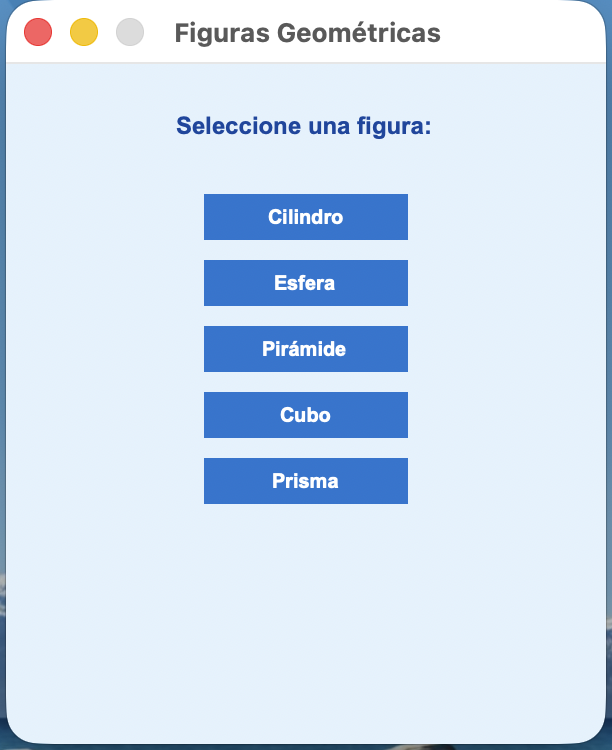
\includegraphics[width=0.38\textwidth]{img/figuras_menu.png}
    \caption{Menú principal con las cinco figuras geométricas disponibles.}
\end{figure}

\begin{figure}[H]
    \centering
    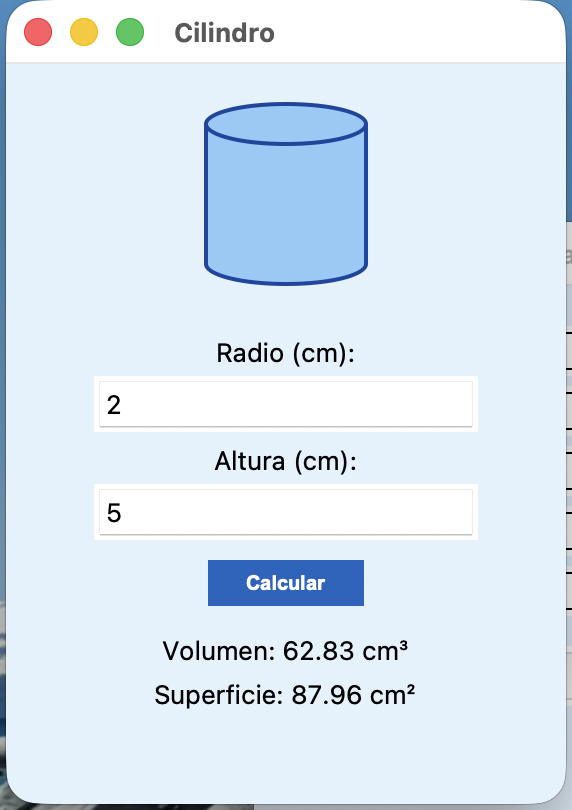
\includegraphics[width=0.31\textwidth]{img/figura_cilindro.png}
    \hspace{0.02\textwidth}
    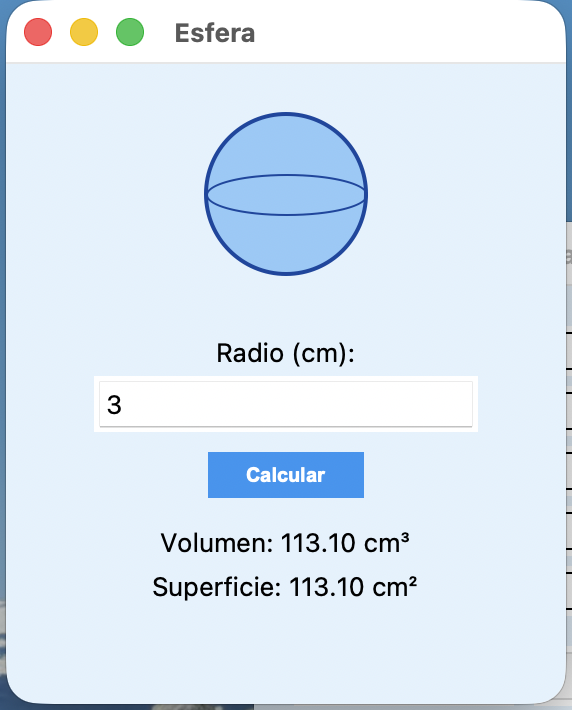
\includegraphics[width=0.31\textwidth]{img/figura_esfera.png}
    \hspace{0.02\textwidth}
    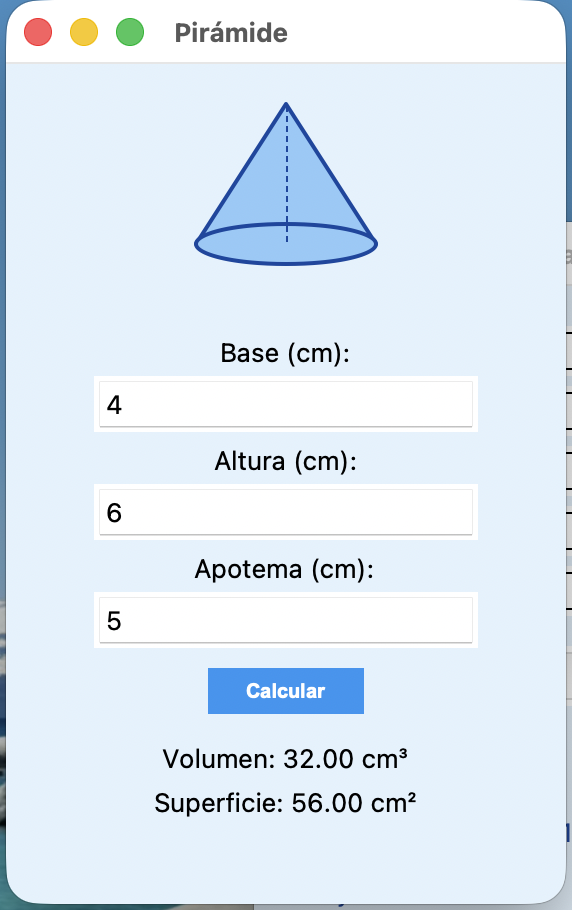
\includegraphics[width=0.31\textwidth]{img/figura_piramide.png}
    \caption{Ventanas del cilindro, la esfera y la pirámide, cada una con su imagen
             y sus resultados.}
\end{figure}

\begin{figure}[H]
    \centering
    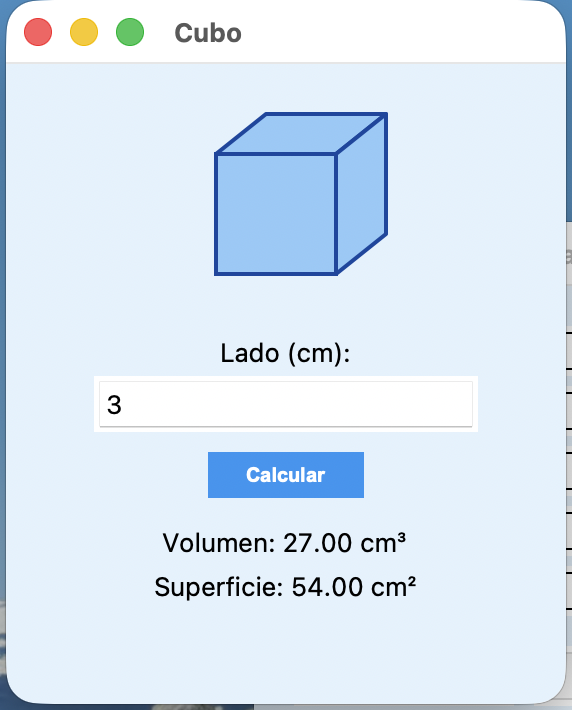
\includegraphics[width=0.31\textwidth]{img/figura_cubo.png}
    \hspace{0.02\textwidth}
    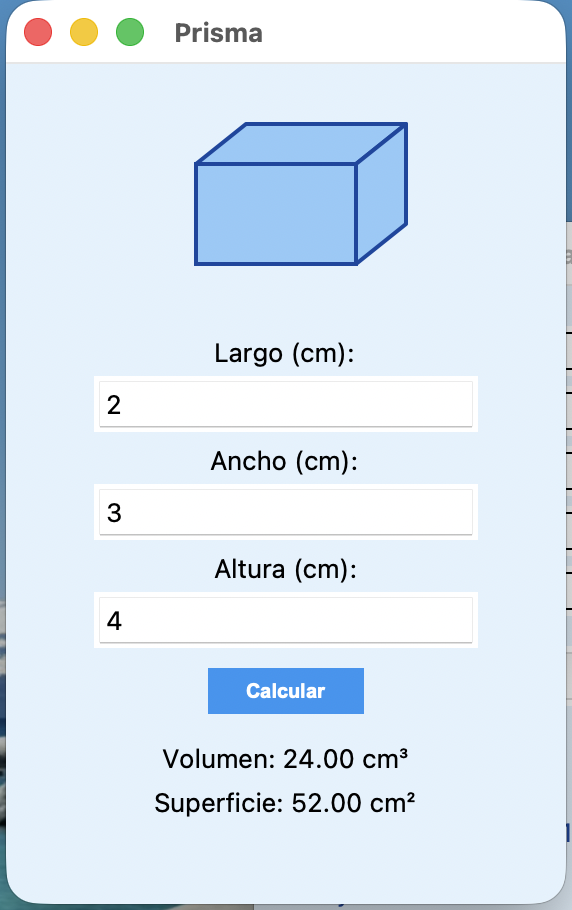
\includegraphics[width=0.31\textwidth]{img/figura_prisma.png}
    \caption{Ventanas del cubo y del prisma, figuras agregadas como parte de los
             ejercicios propuestos.}
\end{figure}

\subsection{Código fuente}
\begin{lstlisting}
import tkinter as tk
from tkinter import messagebox, ttk
import math

# ==========================================
# JERARQUÍA DE CLASES (Lógica del Negocio)
# ==========================================

class FiguraGeometrica:
    """Clase base que almacena los resultados de los cálculos."""
    def __init__(self):
        self.volumen = 0.0
        self.superficie = 0.0

    def get_volumen(self):
        return self.volumen

    def get_superficie(self):
        return self.superficie

class Cilindro(FiguraGeometrica):
    def __init__(self, radio, altura):
        super().__init__()
        self.radio = radio
        self.altura = altura
        self.calcular_volumen()
        self.calcular_superficie()

    def calcular_volumen(self):
        # Fórmula: π * r² * h
        self.volumen = math.pi * (self.radio ** 2) * self.altura

    def calcular_superficie(self):
        # Fórmula: 2πrh + 2πr²
        self.superficie = (2 * math.pi * self.radio * self.altura) + (2 * math.pi * (self.radio ** 2))

class Esfera(FiguraGeometrica):
    def __init__(self, radio):
        super().__init__()
        self.radio = radio
        self.calcular_volumen()
        self.calcular_superficie()

    def calcular_volumen(self):
        # Fórmula: 4/3 * π * r³
        self.volumen = (4.0 / 3.0) * math.pi * (self.radio ** 3)

    def calcular_superficie(self):
        # Fórmula: 4 * π * r²
        self.superficie = 4.0 * math.pi * (self.radio ** 2)

class Piramide(FiguraGeometrica):
    def __init__(self, base, altura, apotema):
        super().__init__()
        self.base = base
        self.altura = altura
        self.apotema = apotema
        self.calcular_volumen()
        self.calcular_superficie()

    def calcular_volumen(self):
        # Fórmula: (base² * altura) / 3
        self.volumen = ((self.base ** 2) * self.altura) / 3.0

    def calcular_superficie(self):
        # Fórmula: base² + 2 * base * apotema
        self.superficie = (self.base ** 2) + (2.0 * self.base * self.apotema)

class Cubo(FiguraGeometrica):
    def __init__(self, lado):
        super().__init__()
        self.lado = lado
        self.calcular_volumen()
        self.calcular_superficie()

    def calcular_volumen(self):
        # Fórmula: lado³
        self.volumen = self.lado ** 3

    def calcular_superficie(self):
        # Fórmula: 6 * lado²
        self.superficie = 6.0 * (self.lado ** 2)

class Prisma(FiguraGeometrica):
    """Prisma rectangular definido por su largo, ancho y altura."""
    def __init__(self, largo, ancho, altura):
        super().__init__()
        self.largo = largo
        self.ancho = ancho
        self.altura = altura
        self.calcular_volumen()
        self.calcular_superficie()

    def calcular_volumen(self):
        # Fórmula: largo * ancho * altura
        self.volumen = self.largo * self.ancho * self.altura

    def calcular_superficie(self):
        # Fórmula: 2 * (largo*ancho + largo*altura + ancho*altura)
        self.superficie = 2.0 * ((self.largo * self.ancho) +
                                 (self.largo * self.altura) +
                                 (self.ancho * self.altura))


# ==========================================
# IMÁGENES DE LAS FIGURAS (dibujadas con Canvas)
# ==========================================

COLOR_FONDO = "#e3f2fd"
COLOR_BORDE = "#0d47a1"
COLOR_RELLENO = "#90caf9"

def configurar_estilos(ventana):
    """Define el estilo azul de los botones.

    Se usa ttk con el tema "clam" porque los botones tk no admiten colores
    de fondo en macOS y el texto blanco quedaría ilegible.
    """
    estilo = ttk.Style(ventana)
    estilo.theme_use("clam")
    estilo.configure("Menu.TButton", background="#1976d2", foreground="white",
                     font=("Arial", 10, "bold"), borderwidth=0, focuscolor="#1976d2")
    estilo.map("Menu.TButton", background=[("active", "#0d47a1")])
    estilo.configure("Calcular.TButton", background="#2196f3", foreground="white",
                     font=("Arial", 10, "bold"), borderwidth=0, focuscolor="#2196f3")
    estilo.map("Calcular.TButton", background=[("active", "#1565c0")])

def dibujar_figura(canvas, tipo):
    """Dibuja sobre el canvas la imagen de la figura geométrica indicada."""
    estilo = {"outline": COLOR_BORDE, "fill": COLOR_RELLENO, "width": 2}

    if tipo == "cilindro":
        canvas.create_oval(40, 85, 120, 105, **estilo)
        canvas.create_rectangle(40, 25, 120, 95, outline="", fill=COLOR_RELLENO)
        canvas.create_line(40, 25, 40, 95, fill=COLOR_BORDE, width=2)
        canvas.create_line(120, 25, 120, 95, fill=COLOR_BORDE, width=2)
        canvas.create_oval(40, 15, 120, 35, **estilo)

    elif tipo == "esfera":
        canvas.create_oval(40, 20, 120, 100, **estilo)
        canvas.create_oval(40, 50, 120, 70, outline=COLOR_BORDE, width=1)

    elif tipo == "piramide":
        canvas.create_polygon(80, 15, 35, 85, 125, 85,
                              outline=COLOR_BORDE, fill=COLOR_RELLENO, width=2)
        canvas.create_oval(35, 75, 125, 95, outline=COLOR_BORDE, fill=COLOR_RELLENO, width=2)
        canvas.create_line(80, 15, 80, 85, fill=COLOR_BORDE, width=1, dash=(3, 2))

    elif tipo == "cubo":
        canvas.create_polygon(45, 40, 70, 20, 130, 20, 105, 40,
                              outline=COLOR_BORDE, fill=COLOR_RELLENO, width=2)
        canvas.create_polygon(105, 40, 130, 20, 130, 80, 105, 100,
                              outline=COLOR_BORDE, fill=COLOR_RELLENO, width=2)
        canvas.create_rectangle(45, 40, 105, 100, **estilo)

    elif tipo == "prisma":
        canvas.create_polygon(35, 45, 60, 25, 140, 25, 115, 45,
                              outline=COLOR_BORDE, fill=COLOR_RELLENO, width=2)
        canvas.create_polygon(115, 45, 140, 25, 140, 75, 115, 95,
                              outline=COLOR_BORDE, fill=COLOR_RELLENO, width=2)
        canvas.create_rectangle(35, 45, 115, 95, **estilo)


# ==========================================
# INTERFAZ GRÁFICA (Tkinter)
# ==========================================

class VentanaPrincipal(tk.Tk):
    def __init__(self):
        super().__init__()
        self.title("Figuras Geométricas")
        self.geometry("300x340")
        self.configure(bg=COLOR_FONDO) # Fondo azul claro
        self.resizable(False, False)
        self.eval('tk::PlaceWindow . center')

        # Estilo para botones
        configurar_estilos(self)
        btn_style = {"width": 15, "style": "Menu.TButton"}

        tk.Label(self, text="Seleccione una figura:", font=("Arial", 12, "bold"),
                 bg=COLOR_FONDO, fg=COLOR_BORDE).pack(pady=20)

        ttk.Button(self, text="Cilindro", command=self.abrir_cilindro, **btn_style).pack(pady=5)
        ttk.Button(self, text="Esfera", command=self.abrir_esfera, **btn_style).pack(pady=5)
        ttk.Button(self, text="Pirámide", command=self.abrir_piramide, **btn_style).pack(pady=5)
        ttk.Button(self, text="Cubo", command=self.abrir_cubo, **btn_style).pack(pady=5)
        ttk.Button(self, text="Prisma", command=self.abrir_prisma, **btn_style).pack(pady=5)

    def abrir_cilindro(self): VentanaCilindro(self)
    def abrir_esfera(self): VentanaEsfera(self)
    def abrir_piramide(self): VentanaPiramide(self)
    def abrir_cubo(self): VentanaCubo(self)
    def abrir_prisma(self): VentanaPrisma(self)

class VentanaFigura(tk.Toplevel):
    """Ventana base: muestra la imagen de la figura y sus campos de entrada."""
    def __init__(self, parent, titulo, tipo, etiquetas, alto):
        super().__init__(parent)
        self.title(titulo)
        self.geometry(f"280x{alto}")
        self.configure(bg=COLOR_FONDO)

        # Imagen de la figura geométrica
        canvas = tk.Canvas(self, width=160, height=120, bg=COLOR_FONDO, highlightthickness=0)
        canvas.pack(pady=5)
        dibujar_figura(canvas, tipo)

        # Un campo de entrada por cada dato solicitado
        self.entradas = []
        for etiqueta in etiquetas:
            tk.Label(self, text=etiqueta, bg=COLOR_FONDO).pack(pady=2)
            txt_entry = tk.Entry(self)
            txt_entry.pack()
            self.entradas.append(txt_entry)

        ttk.Button(self, text="Calcular", command=self.calcular,
                   style="Calcular.TButton").pack(pady=10)

        self.lbl_volumen = tk.Label(self, text="Volumen: ", bg=COLOR_FONDO)
        self.lbl_volumen.pack()
        self.lbl_superficie = tk.Label(self, text="Superficie: ", bg=COLOR_FONDO)
        self.lbl_superficie.pack()

    def crear_figura(self, valores):
        """Cada ventana construye su propia figura con los valores ingresados."""
        raise NotImplementedError

    def calcular(self):
        try:
            valores = [float(entrada.get()) for entrada in self.entradas]
            figura = self.crear_figura(valores)
            self.lbl_volumen.config(text=f"Volumen: {figura.get_volumen():.2f} cm³")
            self.lbl_superficie.config(text=f"Superficie: {figura.get_superficie():.2f} cm²")
        except ValueError:
            messagebox.showerror("Error", "Ingrese valores numéricos válidos.")

class VentanaCilindro(VentanaFigura):
    def __init__(self, parent):
        super().__init__(parent, "Cilindro", "cilindro",
                         ["Radio (cm):", "Altura (cm):"], 370)

    def crear_figura(self, valores):
        return Cilindro(valores[0], valores[1])

class VentanaEsfera(VentanaFigura):
    def __init__(self, parent):
        super().__init__(parent, "Esfera", "esfera",
                         ["Radio (cm):"], 320)

    def crear_figura(self, valores):
        return Esfera(valores[0])

class VentanaPiramide(VentanaFigura):
    def __init__(self, parent):
        super().__init__(parent, "Pirámide", "piramide",
                         ["Base (cm):", "Altura (cm):", "Apotema (cm):"], 420)

    def crear_figura(self, valores):
        return Piramide(valores[0], valores[1], valores[2])

class VentanaCubo(VentanaFigura):
    def __init__(self, parent):
        super().__init__(parent, "Cubo", "cubo",
                         ["Lado (cm):"], 320)

    def crear_figura(self, valores):
        return Cubo(valores[0])

class VentanaPrisma(VentanaFigura):
    def __init__(self, parent):
        super().__init__(parent, "Prisma", "prisma",
                         ["Largo (cm):", "Ancho (cm):", "Altura (cm):"], 420)

    def crear_figura(self, valores):
        return Prisma(valores[0], valores[1], valores[2])

if __name__ == "__main__":
    app = VentanaPrincipal()
    app.mainloop()
\end{lstlisting}

\end{document}
